%%% Template para Relatório Técnico - UTFPR
%%% Baseado no template de Willian Chamma / Mikhail Klassen

\documentclass[12pt,a4paper, brazil]{article}

%%%%%%% INFORMAÇÕES DO CABEÇALHO
\newcommand{\workingDate}{\textsc{\selectlanguage{portuguese}\today}}
\newcommand{\userName}{LRCO7A}
\newcommand{\institution}{UTFPR-AP}
\usepackage{researchdiary_png}

\usepackage{listings}
\usepackage{float}
\usepackage{placeins}

% Configuração para código VHDL
\lstdefinestyle{vhdl}{
    language=VHDL,
    basicstyle=\ttfamily\small,
    keywordstyle=\color{blue}\bfseries,
    commentstyle=\color{gray}\itshape,
    stringstyle=\color{red},
    numbers=left,
    numberstyle=\tiny\color{gray},
    numbersep=5pt,
    frame=single,
    breaklines=true,
    captionpos=b,
    tabsize=2
}

\begin{document}

\begin{center}
{\textbf {\huge Atividade Prática 2 -- Introdução à placa DE10-Lite}}\\[5mm]
{\large Pedro Lucas dos Reis Silva - RA: 2272040} \\[5mm]
02/04/2026\\[5mm]
\end{center}

% ============================================================
\section{Introdução}
% ============================================================

Esta atividade tem como objetivo a introdução à placa FPGA DE10-Lite, realizando a implementação de circuitos combinacionais em hardware real. A atividade é composta por dois exercícios:

\begin{enumerate}
    \item Implementação das 8 portas lógicas (conforme Atividade 1) na placa DE10-Lite, utilizando chaves (slide switches) como entradas e LEDs como saídas.
    \item Projeto de um circuito de controle para uma máquina de cópias, que detecta quando duas ou mais chaves estão fechadas simultaneamente, utilizando simplificação por mapa de Karnaugh.
\end{enumerate}

A placa DE10-Lite utiliza o FPGA Intel MAX 10 e possui 10 slide switches (SW0--SW9) e 10 LEDs vermelhos (LEDR0--LEDR9), operando em nível lógico 3.3V LVTTL. O mapeamento entre os pinos lógicos do VHDL e os pinos físicos da placa é feito através do \textit{Pin Planner} do Quartus Prime.

Os códigos VHDL completos encontram-se nos Apêndices ao final deste relatório.

% ============================================================
% EXERCÍCIO 1
% ============================================================
\section{Exercício 1 -- Portas Lógicas na DE10-Lite}
% ============================================================

\subsection{Descrição}

Neste exercício, o mesmo circuito desenvolvido na Atividade 1 (8 portas lógicas: NOT a, NOT b, AND, OR, NAND, NOR, XOR, XNOR) foi implementado na placa DE10-Lite. As entradas \texttt{a} e \texttt{b} foram associadas às slide switches SW0 e SW1, e cada saída (z1 a z8) foi associada a um LED.

\subsection{Pin Planner}

A Tabela \ref{tab:pinplan-ex1} apresenta o mapeamento dos pinos utilizado no Quartus Prime para o Exercício 1.

\begin{table}[H]
\centering
\caption{Pin Planner -- Exercício 1 (portas lógicas).}
\label{tab:pinplan-ex1}
\begin{tabular}{@{}llll@{}}
\toprule
\textbf{Sinal} & \textbf{Componente} & \textbf{Pino FPGA} & \textbf{I/O Standard} \\
\midrule
a   & SW0 (Slide Switch 0) & PIN\_C10 & 3.3-V LVTTL \\
b   & SW1 (Slide Switch 1) & PIN\_C11 & 3.3-V LVTTL \\
z1--z8 & LEDR0--LEDR7        & ---      & 3.3-V LVTTL \\
\bottomrule
\end{tabular}
\end{table}

\begin{figure}[H]
    \centering
    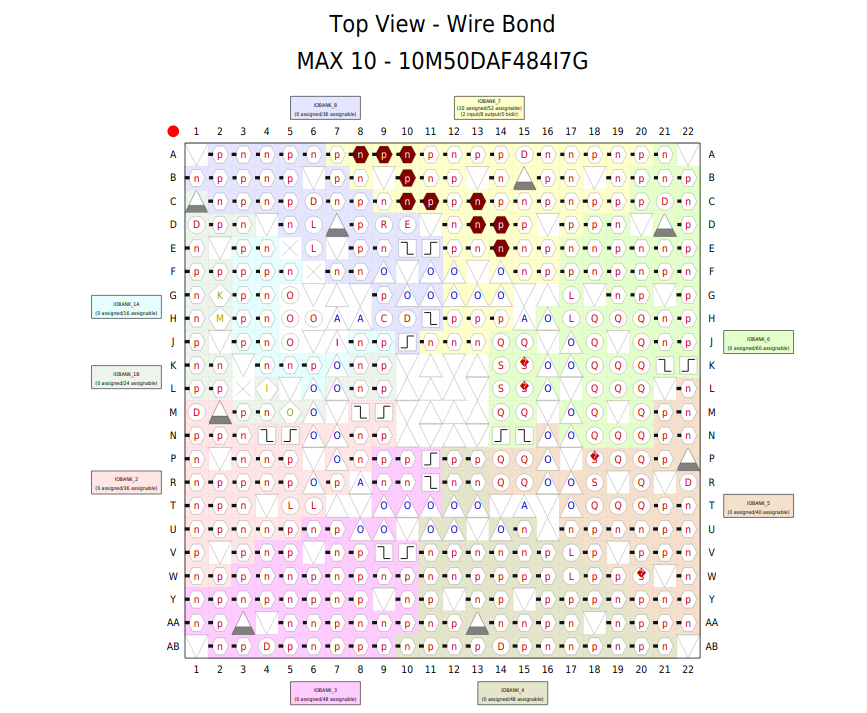
\includegraphics[width=0.95\textwidth]{pinplan-ex1.png}
    \caption{Pin Planner do Exercício 1 no Quartus Prime.}
    \label{fig:pinplan-ex1}
\end{figure}
\FloatBarrier

% ============================================================
% EXERCÍCIO 2
% ============================================================
\section{Exercício 2 -- Circuito de Controle da Máquina de Cópias}
% ============================================================

\subsection{Descrição do Problema}

Quatro chaves (SW1 a SW4) estão posicionadas ao longo do caminho do papel em uma máquina de cópias. Cada chave é normalmente aberta e fecha quando o papel passa por ela. Cada chave possui um resistor de \textit{pull-up} conectado a +5V, garantindo nível lógico alto quando aberta e nível baixo quando fechada. Na placa DE10-Lite, as slide switches já possuem circuito de pull-up integrado operando em 3.3V LVTTL, de modo que a lógica permanece a mesma: chave ativada = \texttt{'1'}, chave desativada = \texttt{'0'}.

O circuito deve produzir saída alta sempre que \textbf{duas ou mais} chaves estejam fechadas ao mesmo tempo. Como restrição do problema, as chaves SW1 e SW4 \textbf{nunca} estarão fechadas simultaneamente, o que permite o uso de condições \textit{don't care} para simplificação.

\subsection{Tabela Verdade}

A Tabela \ref{tab:verdade-ex2} apresenta a tabela verdade completa. As combinações onde SW1=1 e SW4=1 simultaneamente são marcadas como \textit{don't care} (X), pois esse cenário é fisicamente impossível.

\begin{table}[H]
\centering
\caption{Tabela verdade do circuito de controle -- saída z=1 quando 2 ou mais chaves fechadas.}
\label{tab:verdade-ex2}
\begin{tabular}{@{}cccc|c|l@{}}
\toprule
\textbf{SW1} & \textbf{SW2} & \textbf{SW3} & \textbf{SW4} & \textbf{z} & \textbf{Observação} \\
\midrule
0 & 0 & 0 & 0 & 0 & Nenhuma chave fechada \\
0 & 0 & 0 & 1 & 0 & Apenas 1 chave \\
0 & 0 & 1 & 0 & 0 & Apenas 1 chave \\
0 & 0 & 1 & 1 & 1 & SW3 + SW4 \\
0 & 1 & 0 & 0 & 0 & Apenas 1 chave \\
0 & 1 & 0 & 1 & 1 & SW2 + SW4 \\
0 & 1 & 1 & 0 & 1 & SW2 + SW3 \\
0 & 1 & 1 & 1 & 1 & SW2 + SW3 + SW4 \\
1 & 0 & 0 & 0 & 0 & Apenas 1 chave \\
1 & 0 & 0 & 1 & X & \textit{don't care} (SW1+SW4 impossível) \\
1 & 0 & 1 & 0 & 1 & SW1 + SW3 \\
1 & 0 & 1 & 1 & X & \textit{don't care} \\
1 & 1 & 0 & 0 & 1 & SW1 + SW2 \\
1 & 1 & 0 & 1 & X & \textit{don't care} \\
1 & 1 & 1 & 0 & 1 & SW1 + SW2 + SW3 \\
1 & 1 & 1 & 1 & X & \textit{don't care} \\
\bottomrule
\end{tabular}
\end{table}
\FloatBarrier

\subsection{Mapa de Karnaugh}

A tabela verdade foi transposta para o mapa de Karnaugh de 4 variáveis, com SW1$\cdot$SW2 nas linhas e SW3$\cdot$SW4 nas colunas (ordenação Gray):

\begin{table}[H]
\centering
\caption{Mapa de Karnaugh -- agrupamentos para simplificação.}
\label{tab:karnaugh}
\begin{tabular}{c|c|c|c|c|}
\cline{2-5}
 & \multicolumn{4}{c|}{\textbf{SW3$\cdot$SW4}} \\
\cline{2-5}
\textbf{SW1$\cdot$SW2} & \textbf{00} & \textbf{01} & \textbf{11} & \textbf{10} \\
\hline
\multicolumn{1}{|c|}{\textbf{00}} & 0 & 0 & 1 & 0 \\
\hline
\multicolumn{1}{|c|}{\textbf{01}} & 0 & 1 & 1 & 1 \\
\hline
\multicolumn{1}{|c|}{\textbf{11}} & 1 & X & X & 1 \\
\hline
\multicolumn{1}{|c|}{\textbf{10}} & 0 & X & X & 1 \\
\hline
\end{tabular}
\end{table}

Os agrupamentos identificados (incluindo \textit{don't cares} para maximizar os grupos) são:

\begin{enumerate}
    \item \textbf{SW3$\cdot$SW4}: cobre as células (00,11), (01,11), (11,11), (10,11)
    \item \textbf{SW2$\cdot$SW4}: cobre as células (01,01), (01,11), (11,01), (11,11)
    \item \textbf{SW2$\cdot$SW3}: cobre as células (01,10), (01,11), (11,10), (11,11)
    \item \textbf{SW1$\cdot$SW2}: cobre as células (11,00), (11,01), (11,10), (11,11)
    \item \textbf{SW1$\cdot$SW3}: cobre as células (10,10), (10,11), (11,10), (11,11)
\end{enumerate}

\subsection{Equação Booleana Simplificada}

A equação mínima em soma de produtos obtida é:

\begin{equation}
\boxed{z = SW1 \cdot SW2 + SW1 \cdot SW3 + SW2 \cdot SW3 + SW2 \cdot SW4 + SW3 \cdot SW4}
\label{eq:booleana}
\end{equation}

Note que o termo $SW1 \cdot SW4$ não aparece na equação, pois essa combinação é fisicamente impossível (condição \textit{don't care}) e foi aproveitada para simplificar os demais agrupamentos.

\subsection{Implementação VHDL}

A equação \eqref{eq:booleana} foi implementada diretamente em VHDL no estilo \textit{dataflow}, com uma única atribuição concorrente (ver Apêndice \ref{ap:codigo-ex2}). Cada termo da equação corresponde a um par de chaves que, quando ambas fechadas, ativa a saída.

\subsection{Pin Planner}

A Tabela \ref{tab:pinplan-ex2} apresenta o mapeamento dos pinos utilizado no Quartus Prime para o Exercício 2.

\begin{table}[H]
\centering
\caption{Pin Planner -- Exercício 2 (máquina de cópias).}
\label{tab:pinplan-ex2}
\begin{tabular}{@{}llll@{}}
\toprule
\textbf{Sinal} & \textbf{Componente} & \textbf{Pino FPGA} & \textbf{I/O Standard} \\
\midrule
chave1 (SW1) & SW0 (Slide Switch 0) & PIN\_C10 & 3.3-V LVTTL \\
chave2 (SW2) & SW1 (Slide Switch 1) & PIN\_C11 & 3.3-V LVTTL \\
chave3 (SW3) & SW2 (Slide Switch 2) & PIN\_D12 & 3.3-V LVTTL \\
chave4 (SW4) & SW3 (Slide Switch 3) & PIN\_C12 & 3.3-V LVTTL \\
z (saída)    & LEDR0 (LED Vermelho) & PIN\_A8  & 3.3-V LVTTL \\
\bottomrule
\end{tabular}
\end{table}

\begin{figure}[H]
    \centering
    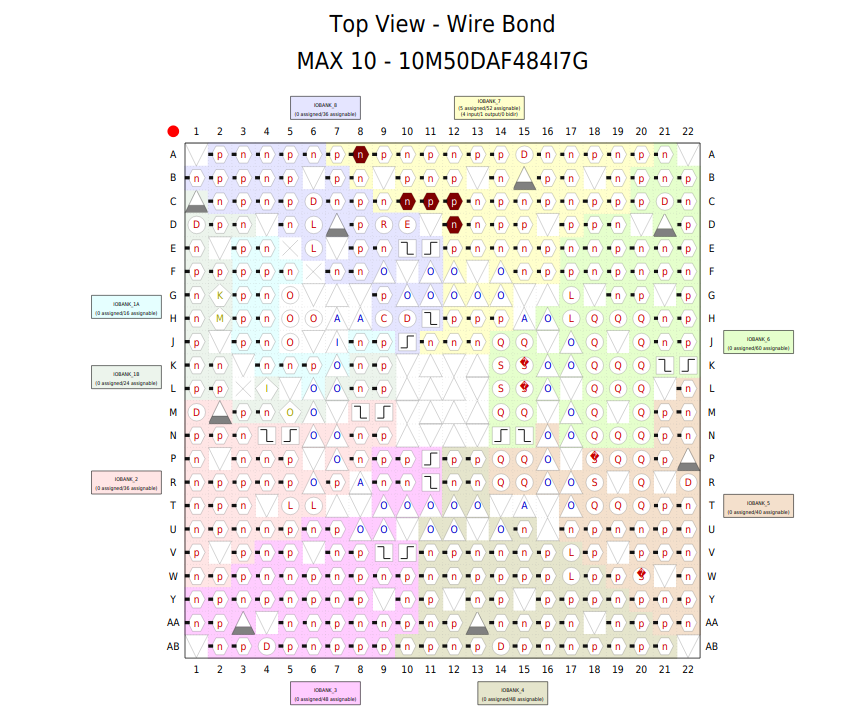
\includegraphics[width=0.95\textwidth]{pinplan-ex2.png}
    \caption{Pin Planner do Exercício 2 no Quartus Prime.}
    \label{fig:pinplan-ex2}
\end{figure}
\FloatBarrier

\subsection{Simulação}

A simulação foi realizada no Quartus Prime, testando todas as 16 combinações possíveis das 4 chaves. A Figura \ref{fig:sim-ex2} apresenta as formas de onda obtidas. Observa-se que a saída \texttt{z} vai para nível alto somente quando duas ou mais chaves estão ativadas.

Nas combinações onde SW1=1 e SW4=1 simultaneamente (condições \textit{don't care}), a saída também resulta em nível alto. Isso é esperado: no mapa de Karnaugh, essas condições foram tratadas como \texttt{'1'} para permitir agrupamentos maiores e obter uma equação mais simples. Como essa combinação de entrada é fisicamente impossível na máquina de cópias, o valor da saída nesse caso é irrelevante --- poderia ser 0 ou 1 sem afetar o funcionamento real do circuito.

\begin{figure}[H]
    \centering
    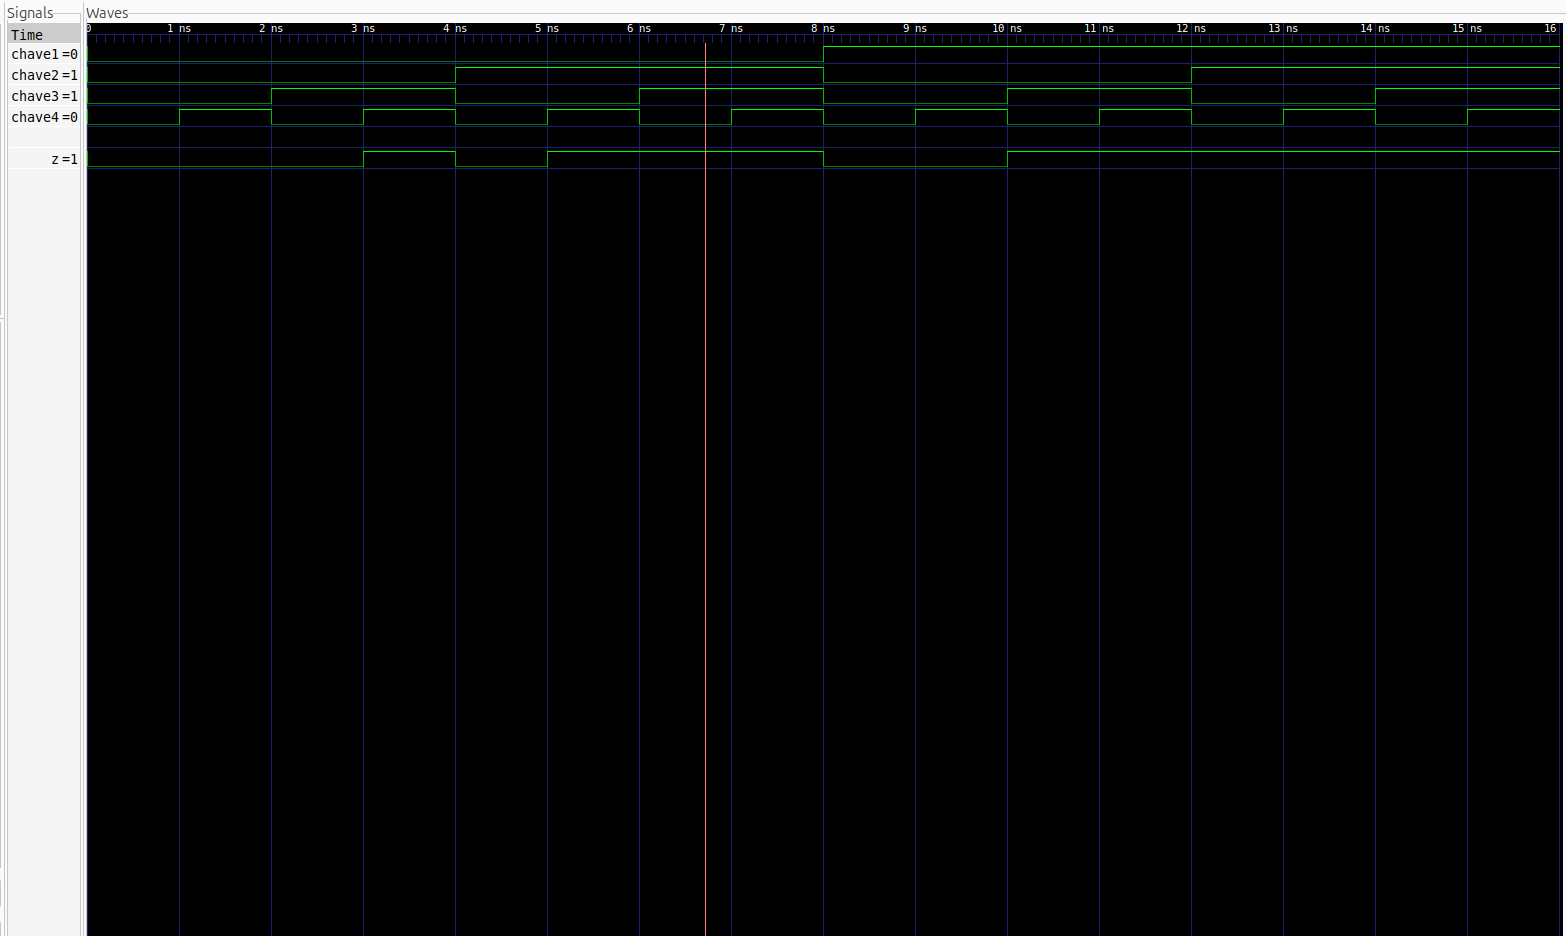
\includegraphics[width=0.95\textwidth]{sim-ex2.png}
    \caption{Simulação do circuito de controle da máquina de cópias no Quartus Prime.}
    \label{fig:sim-ex2}
\end{figure}
\FloatBarrier

\subsection{Diagrama RTL}

O diagrama RTL foi gerado pelo Quartus Prime através da ferramenta \textit{RTL Viewer} (Tools $\rightarrow$ Netlist Viewers $\rightarrow$ RTL Viewer). A Figura \ref{fig:rtl-ex2} apresenta a estrutura do circuito sintetizado, onde se observam as portas AND de 2 entradas e a porta OR combinando os 5 termos da equação simplificada.

\begin{figure}[H]
    \centering
    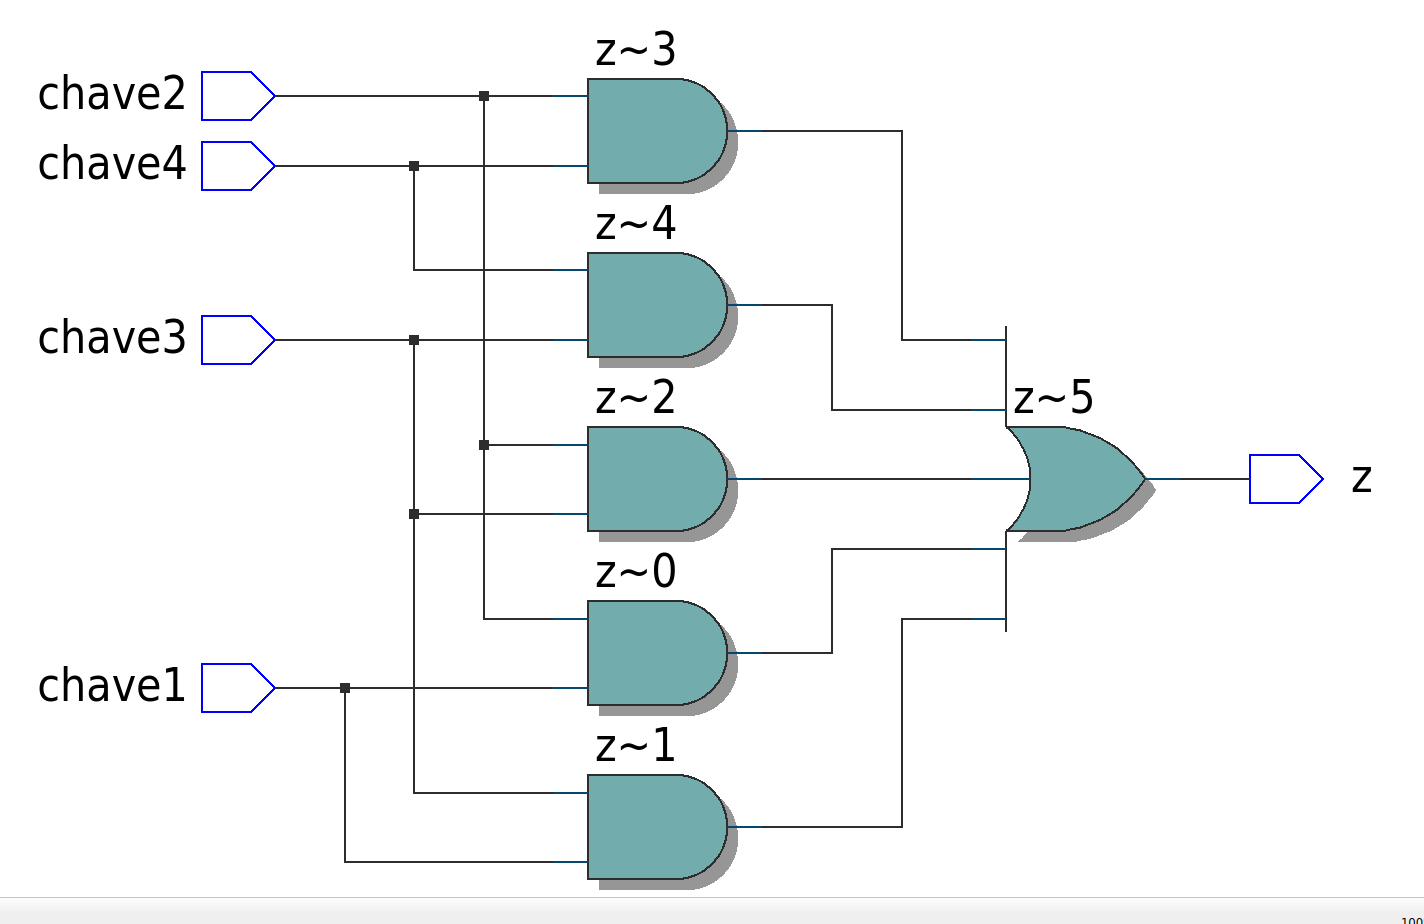
\includegraphics[width=0.95\textwidth]{rtl-ex2.png}
    \caption{Diagrama RTL do circuito de controle, gerado pelo Quartus Prime.}
    \label{fig:rtl-ex2}
\end{figure}
\FloatBarrier

% ============================================================
\section{Considerações Finais}
% ============================================================

Ambos os exercícios foram implementados com sucesso na placa DE10-Lite. No Exercício 1, as 8 portas lógicas responderam corretamente às combinações de entrada através das slide switches, com os LEDs indicando os resultados esperados. No Exercício 2, o circuito de controle da máquina de cópias detectou corretamente quando duas ou mais chaves estavam fechadas, acendendo o LED correspondente.

O uso do mapa de Karnaugh no Exercício 2 permitiu obter uma equação simplificada com 5 termos de produto, aproveitando as condições \textit{don't care} da restrição $SW1 \cdot SW4 = 0$ para reduzir a complexidade do circuito.

O Quartus Prime mostrou-se a ferramenta adequada para esta etapa do desenvolvimento, realizando a síntese, o mapeamento de pinos e a gravação na placa FPGA. A simulação e a geração do diagrama RTL foram realizadas diretamente no Quartus. Para as atividades anteriores, a simulação foi feita com ferramentas open source (GHDL + GTKWave) em ambiente Linux, o que se mostrou viável para verificação funcional antes da síntese no Quartus.

% ============================================================
\appendix
% ============================================================

\newpage
\section{Código VHDL -- Exercício 1 (Portas Lógicas)}
\label{ap:codigo-ex1}

\begin{lstlisting}[style=vhdl, caption={Arquivo atividade1.vhd -- 8 portas lógicas na DE10-Lite.}]
-- ============================================================
-- Atividade 2 - Exercicio 1: Portas Logicas na DE10-Lite
-- Pin Planner: a=SW0(PIN_C10), b=SW1(PIN_C11), z1..z8=LEDR
-- ============================================================
library ieee;
use ieee.std_logic_1164.all;

entity atividade1 is
  port (
    a    : in  bit;   -- SW0: entrada A
    b    : in  bit;   -- SW1: entrada B
    z1   : out bit;   -- LEDR0: NOT a
    z2   : out bit;   -- LEDR1: NOT b
    z3   : out bit;   -- LEDR2: AND
    z4   : out bit;   -- LEDR3: OR
    z5   : out bit;   -- LEDR4: NAND
    z6   : out bit;   -- LEDR5: NOR
    z7   : out bit;   -- LEDR6: XOR
    z8   : out bit    -- LEDR7: XNOR
  );
end entity;

architecture dataflow of atividade1 is
begin
  z1 <= not a;        -- inversao de A
  z2 <= not b;        -- inversao de B
  z3 <= a and b;      -- AND
  z4 <= a or b;       -- OR
  z5 <= a nand b;     -- NAND
  z6 <= a nor b;      -- NOR
  z7 <= a xor b;      -- XOR
  z8 <= a xnor b;     -- XNOR
end architecture;
\end{lstlisting}

\newpage
\section{Código VHDL -- Exercício 2 (Máquina de Cópias)}
\label{ap:codigo-ex2}

\begin{lstlisting}[style=vhdl, caption={Arquivo atividade2.vhd -- circuito de controle da máquina de cópias.}]
-- ============================================================
-- Atividade 2 - Exercicio 2: Circuito de controle maquina de copias
-- Saida HIGH quando 2 ou mais chaves estao fechadas.
-- SW1 e SW4 nunca fecham ao mesmo tempo (don't care).
--
-- Equacao (Karnaugh):
-- z = SW1.SW2 + SW1.SW3 + SW2.SW3 + SW2.SW4 + SW3.SW4
--
-- Pin Planner (DE10-Lite):
--   chave1=SW0(PIN_C10), chave2=SW1(PIN_C11),
--   chave3=SW2(PIN_D12), chave4=SW3(PIN_C12),
--   z=LEDR0(PIN_A8)
-- ============================================================
library ieee;
use ieee.std_logic_1164.all;

entity atividade2 is
  port (
    chave1 : in  bit;  -- SW0: chave 1
    chave2 : in  bit;  -- SW1: chave 2
    chave3 : in  bit;  -- SW2: chave 3
    chave4 : in  bit;  -- SW3: chave 4
    z      : out bit   -- LEDR0: saida
  );
end entity;

architecture dataflow of atividade2 is
begin
  -- Equacao simplificada via Karnaugh
  -- (todas as combinacoes de 2 chaves, exceto
  --  SW1.SW4 que e don't care)
  z <= (chave1 and chave2) or
       (chave1 and chave3) or
       (chave2 and chave3) or
       (chave2 and chave4) or
       (chave3 and chave4);
end architecture;
\end{lstlisting}

\newpage
\section{Resolução Manuscrita -- Tabela Verdade e Mapa de Karnaugh}
\label{ap:mapa-manuscrito}

A Figura \ref{fig:mapa-manuscrito} apresenta a resolução manuscrita do Exercício 2, contendo a tabela verdade completa com as condições \textit{don't care}, o mapa de Karnaugh em ordenação Gray com os agrupamentos identificados, e a equação booleana simplificada obtida.

\begin{figure}[H]
    \centering
    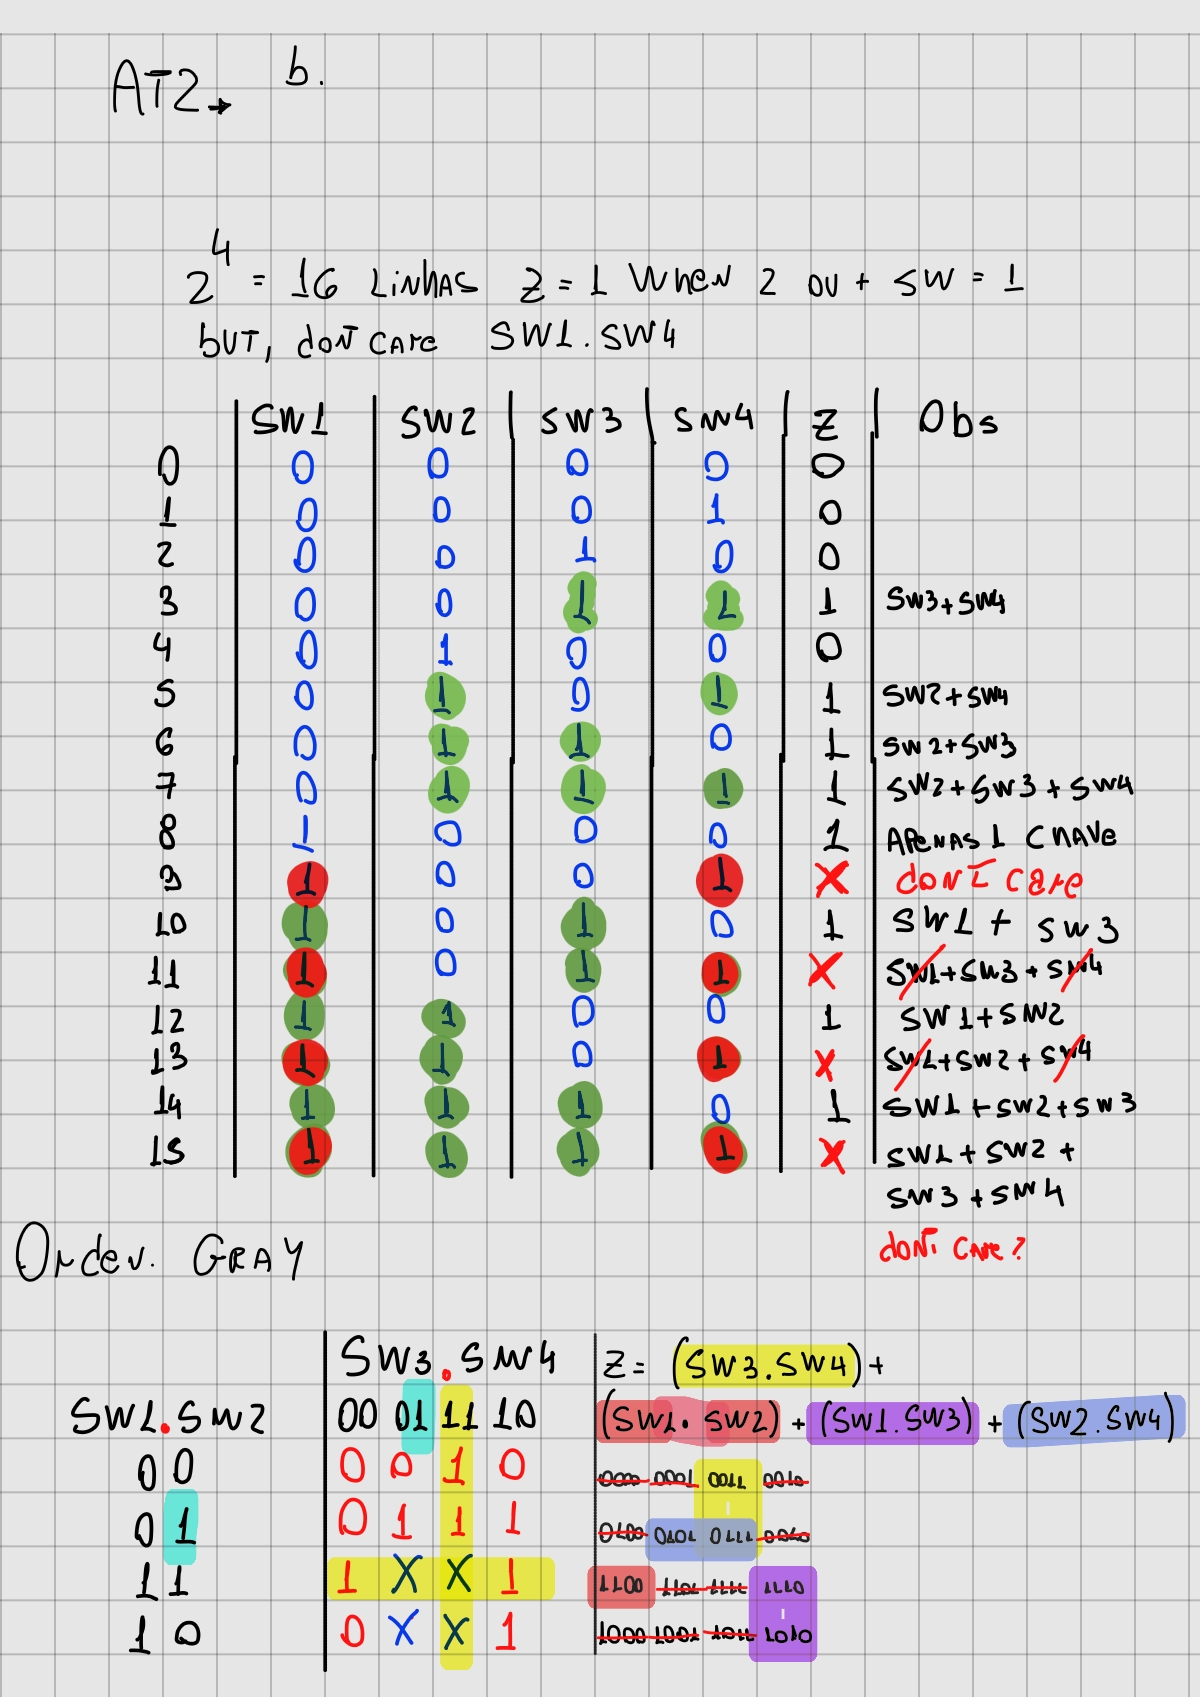
\includegraphics[width=0.75\textwidth]{At2_mapa.jpg}
    \caption{Resolução manuscrita: tabela verdade, mapa de Karnaugh e agrupamentos.}
    \label{fig:mapa-manuscrito}
\end{figure}

\newpage
\section{Código VHDL -- Testbench do Exercício 2}
\label{ap:testbench-ex2}

\begin{lstlisting}[style=vhdl, caption={Arquivo atividade2\_tb.vhd -- testbench com todas as 16 combinações.}]
-- Testbench para atividade2: circuito de controle
-- Testa todas as 16 combinacoes de 4 chaves

entity atividade2_tb is
end entity;

architecture tb of atividade2_tb is
  signal chave1, chave2, chave3, chave4 : bit;
  signal z : bit;
begin
  uut: entity work.atividade2
    port map(
      chave1 => chave1, chave2 => chave2,
      chave3 => chave3, chave4 => chave4,
      z => z
    );

  process
  begin
    chave1<='0'; chave2<='0'; chave3<='0'; chave4<='0'; wait for 1 ns;
    chave1<='0'; chave2<='0'; chave3<='0'; chave4<='1'; wait for 1 ns;
    chave1<='0'; chave2<='0'; chave3<='1'; chave4<='0'; wait for 1 ns;
    chave1<='0'; chave2<='0'; chave3<='1'; chave4<='1'; wait for 1 ns;
    chave1<='0'; chave2<='1'; chave3<='0'; chave4<='0'; wait for 1 ns;
    chave1<='0'; chave2<='1'; chave3<='0'; chave4<='1'; wait for 1 ns;
    chave1<='0'; chave2<='1'; chave3<='1'; chave4<='0'; wait for 1 ns;
    chave1<='0'; chave2<='1'; chave3<='1'; chave4<='1'; wait for 1 ns;
    chave1<='1'; chave2<='0'; chave3<='0'; chave4<='0'; wait for 1 ns;
    chave1<='1'; chave2<='0'; chave3<='0'; chave4<='1'; wait for 1 ns;
    chave1<='1'; chave2<='0'; chave3<='1'; chave4<='0'; wait for 1 ns;
    chave1<='1'; chave2<='0'; chave3<='1'; chave4<='1'; wait for 1 ns;
    chave1<='1'; chave2<='1'; chave3<='0'; chave4<='0'; wait for 1 ns;
    chave1<='1'; chave2<='1'; chave3<='0'; chave4<='1'; wait for 1 ns;
    chave1<='1'; chave2<='1'; chave3<='1'; chave4<='0'; wait for 1 ns;
    chave1<='1'; chave2<='1'; chave3<='1'; chave4<='1'; wait for 1 ns;
    wait;
  end process;
end architecture;
\end{lstlisting}

\end{document}
